\section*{Introduction}

% the separation of sections here is artificial, the body does not have an intro, results nor outro

The $\Lambda$CDM cosmological model has proven extremely effective in
predicting the evolution of our Universe, relying on only six parameters
\cite{Planck2020a}.
In particular, it explains the transition from a predominantly neutral
state in the early stages to the familiar ionized intergalactic medium
(IGM) observed in our relatively nearby surroundings.
This transition is known as cosmic reionization.
Despite a comprehensive understanding of the astrophysical principles
governing this transition, uncertainties persist regarding its precise
timeline \cite{Jin2023}.
The advent of the James Webb Space Telescope (JWST) \cite{Gardner2006}
represents a pivotal moment, substantially bolstering our ability to
directly constrain the evolution of the neutral hydrogen fraction
$x_\HI$.
This progress is being driven by the JWST's enhanced detection
capabilities, enabling the observation of high-redshift quasars
\cite{Eilers2023} and high-redshift galaxies
\cite{Adams2023, Bradley2023, Donnan2023}.

Reionization leads to scattering of Cosmic Microwave Background (CMB)
photons by free electrons, disrupting the CMB angular power spectra
($C_\ell$).
This scattering suppresses the signal at scales smaller than the Hubble
scale at reionization (approximately $\ell>10$) \cite{Planck2020b} due
to the increased\YLtodo{nonzero?} optical depth $\tau_\reio$ \PMCtodo{I hesitate to use nonzero, there is a tiny amount of free electrons that comes from decoupling, I think ``increased''  accurately reflects the physical picture}.
Additionally, it introduces a new signal in the polarization of CMB
photons at large angular scales \cite{Planck2020a}, that is $\propto
\tau_\reio$ in $C^{TE}_\ell$, the cross-correlation of the $E$-mode
polarization with the temperature (intensity), and is $\propto
\tau_\reio^2$ in $C^{EE}_\ell$, the $E$-mode polarization angular auto
power spectrum.
Consequently, heightened sensitivity to CMB polarization becomes crucial
for mitigating the degeneracy between $\tau_\reio$ and other
cosmological parameters, particularly $\As$, the amplitude of the
primordial scalar power spectrum, and $r$, the ratio of tensor-to-scalar
modes \cite{Natale2020}.

While the high-$\ell$ signal holds most of the constraining power for
cosmological parameters, the low-$\ell$ polarization is crucial for
accurately determining $\tau_\reio$\paulo{, particularly through its impact on $C^{EE}_\ell$}.
Hence\YLtodo{connection not obvious to me}, \paulo{How about rephrase: the inclusion of low-$\ell$ -- polarization -- data leads to a lesser degeneracy between $\As$ and $\tau_\reio$ and can diminish the...?} be breaking the degeneracy with $\As$ and diminishing\YLtodo{can diminish?} the influence
of $\tau_\reio$ on other anomalous parameters like $A_\mathrm{lens}$
\cite{Giare2023}.
$A_\mathrm{lens}$ contains information about the expected deflection of
CMB photons due to the underlying matter distribution.
However, interpreting signals at large angular scales (low $\ell$)
without affecting high-$\ell$ measurements has proven challenging. \YLtodo[inline]{need to ask Paulo more about these 2 sentences} This challenge may ultimately require adopting a comprehensive Bayesian
framework to jointly consider cosmology, astrophysics, and instrument
systematics \cite{Paradiso2023}.
\Cref{fig:tau} illustrates current representative constraints on
$\tau_\reio$ \paulo{This paragraph, which should be connected to the ``While...'' but due to the inline comment looks like a separate paragraph, is addressing $\tau_\reio$ measurements/challenges, I feel it is okay.}.\YLtodo{feels a bit out of place here}

\begin{figure}
\centering
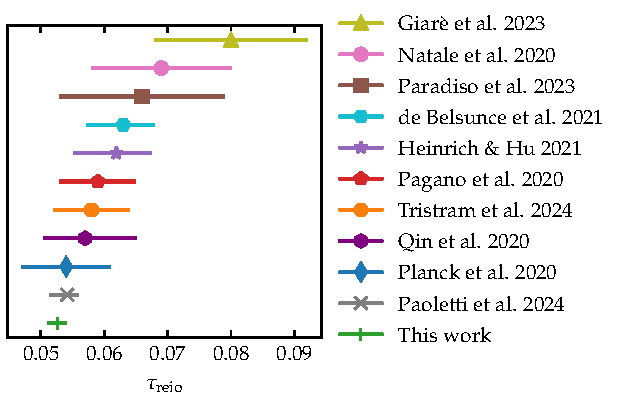
\includegraphics{figs/tau_fig.pdf}
\caption{\textbf{Current constraints on the optical depth to
reionization ($\tau_\reio$) from Cosmic Microwave Background (CMB)
data.}
The error bars indicate the 1$\sigma$ uncertainties.
Various analyses may employ distinct data sets or vary in the parameters
considered.
For instance, the inclusion of WMAP data in Refs.~ \cite{Natale2020,
Paradiso2023} (circle and square) or ACT in combination with other
external data sets \cite{Giare2023} (triangle), expanded sky coverage
\cite{Paradiso2023} (square), incorporation of high-$\ell$ data
\cite{Pagano2020, Planck2020a, Giare2023} (pentagon, star, and
triangle), marginalization over small set of strongly correlated
parameters \cite{Natale2020} (circle), and the implementation of an
end-to-end Bayesian framework that marginalizes over astrophysics and
instrumental systematics \cite{Paradiso2023} (square).}
\label{fig:tau}
\end{figure}

Given the challenges posed by $\tau_\reio$ in CMB analyses and the
anticipated advancements in constraining the reionization timeline
\cite{Montero2021, Hera2022}, now is an opportune moment to reassess its
role.
In theory, cosmic reionization is uniquely determined given a specific
cosmology, i.e.\ by the other five cosmological parameters.
Specifically, the evolution of the global fraction of neutral hydrogen
can be written as
%
\begin{equation}
\label{eq:premise}
x_\HI(a) = f(a; \sigma_8, \ns, h, \Omegab, \Omegam)
\quad \Rightarrow \quad
\tau_\reio = g(\sigma_8, \ns, h, \Omegab, \Omegam),
\end{equation}
%
where $\ns$, $h$, $\Omegab$, and $\Omegam$ are the tilt of the
primordial power spectrum, dimensionless Hubble constant, and present
baryon and matter densities, respectively.
$\sigma_8$ is the present linear rms relative density fluctuation in a
sphere of radius $8 \, h^{-1}\mathrm{Mpc}$.
This parametrization chosen for convenience fully determines $x_\HI$,
but the incomplete understanding of cosmic reionization obscures this
mapping, necessitating the introduction of $\tau_\reio$ in CMB analyses.
However, our understanding of the astrophysical processes governing
reionization has significantly improved \cite{Gnedin2022, Kannan2022,
Murray2020, Fan2023} since the inclusion of $\tau_\reio$ became a
standard practice.
Ongoing and forthcoming observations promise to further our
understanding and reduce inherent modeling uncertainties.
Motivated by these developments, we use symbolic regression (SR)
\cite{Cranmer2023} to construct a mapping between cosmology and
reionization timeline, aiming to demote $\tau_\reio$ from an independent
to a derived cosmological parameter.

Accurately measuring the optical depth to reionization could
significantly tighten cosmological parameter constraints, especially as
$\tau_\reio$ remains the only independent cosmological parameter not
constrained to sub-percent precision \cite{Planck2020b}.
To achieve this precision, sensitivity to E-mode polarization at levels
$\lesssim 10^{-2} \, \mu$K$^2$ and meticulous control of systematic
effects and foregrounds residuals are essential.

\cref{eq:premise} introduces a novel avenue to constrain cosmology
by examining the dependence of $x_\HI(z)$ on cosmological parameters.
This mapping can enhance parameter constraints and shed light on
reionization astrophysics.
It also aids ongoing efforts in parametrizing cosmic reionization models
\cite{Trac2018, Trac2022} by including the cosmological dependence of
$x_\HI$.


\section*{Results}

Here, we present a universality in the neutral hydrogen time evolution,
and derive through SR its dependence on cosmology on simulated
reionization histories from \texttt{21cmFAST} \cite{Murray2020}.
We integrate this shape into \texttt{CLASS} \cite{Blas2011}, a popular
Boltzmann solver for CMB analyses.
We then evaluate the modified \texttt{CLASS} alongside \texttt{Cobaya}
\cite{Torrado2020}, a speed-aware sampler\cite{Lewis2002,
Lewis2013}\footnote{With adaptive covariance learning and fast-dragging
as in \cite{Neal2005}, enabling larger steps in slow parameters via
intermediate transitions of fast parameters.}, showcasing its ability to
recover parameter constraints from CMB data, including `TTTEEE' +
lensing likelihoods \cite{Planck2020c, Planck2020d} (see \Cref{fig:tg}).
Finally, we demonstrate cosmological gains by computing $\tau_\reio$ as
a derived parameter using our approach -- \cref{eq:premise} --
compared to sampling over $\tau_\reio$ using the conventional $\tanh$
model \cite{Lewis2008}.
We summarize our strategy in \Cref{fig:big}.

\begin{figure}
\centering
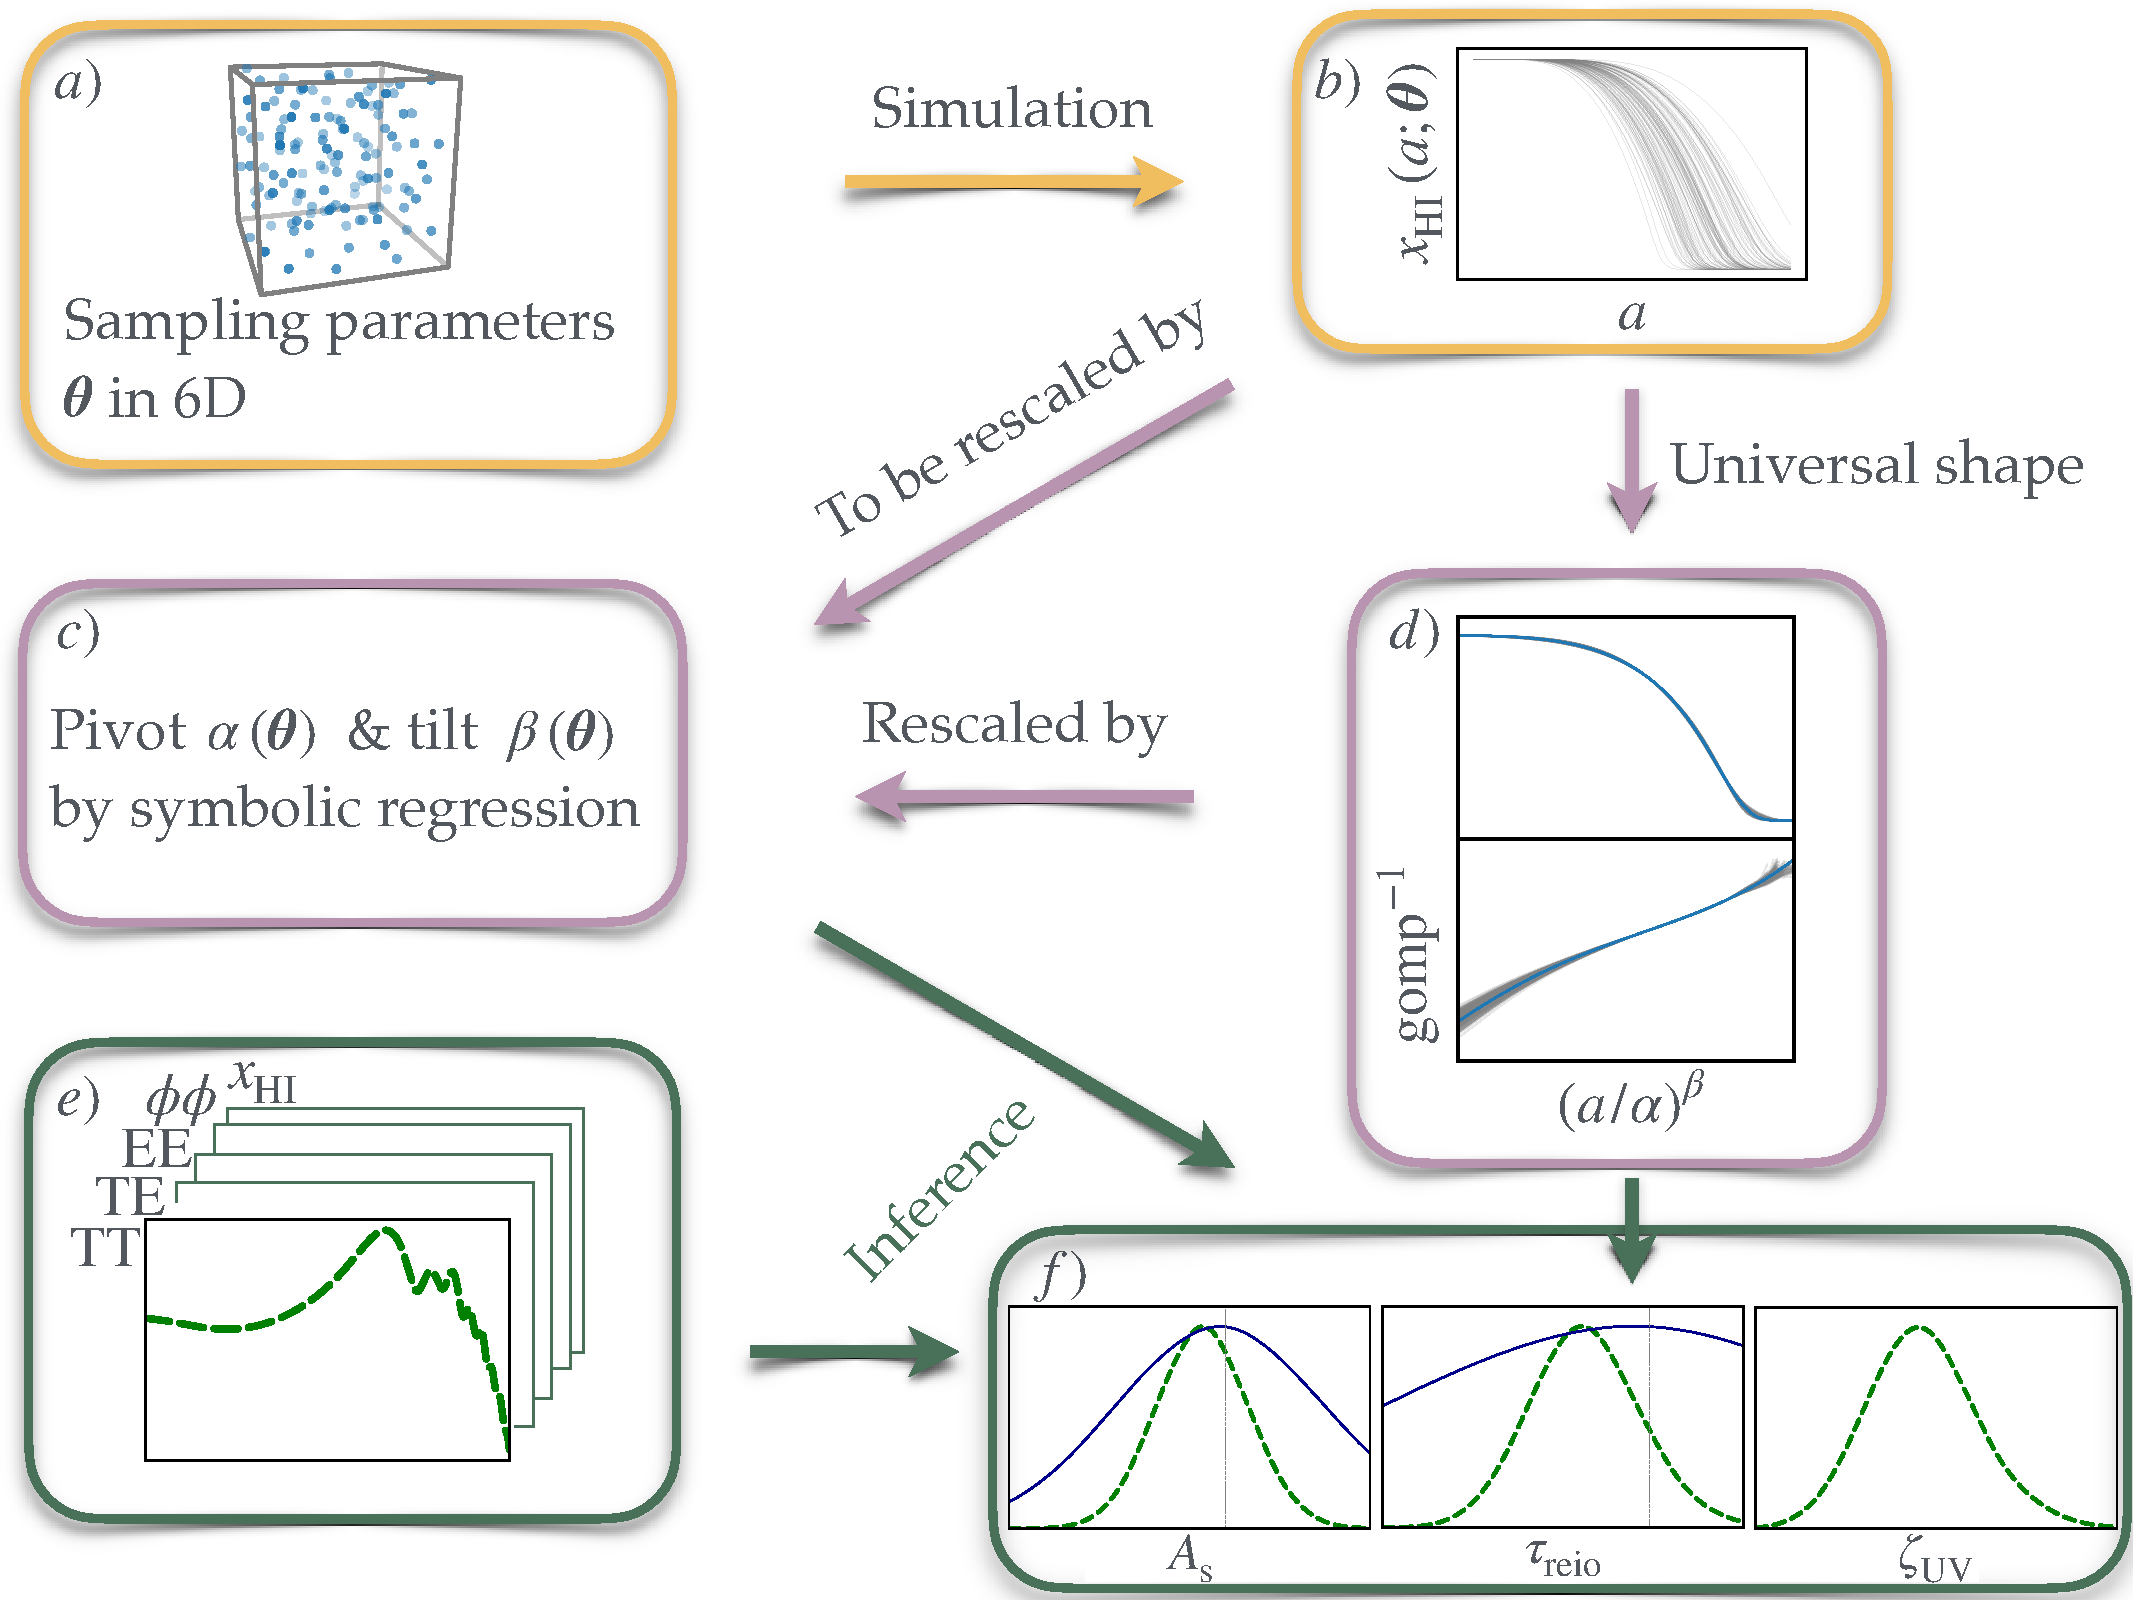
\includegraphics[width=\linewidth]{figs/big_fig.pdf}
\caption{\textbf{Strategy to demote $\tau_\reio$ to derived parameter.}
\emph{a)} Sobol sampling of $\vtheta$ comprising 5 cosmological and 1
astrophysical parameters (see \Cref{fig:sobol} in Extended Data).
\emph{b)} Simulated $x_\HI$ timelines as a function of $\vtheta$ and
scale factor $a$.
\emph{c)} With symbolic regression, we optimize the mapping from
$\vtheta$ to the rescaling parameters that bring the universality.
\emph{d)} We model the universal shape (upper panel) as a composition of
the Gompertz function and a low-degree polynomial (lower panel).
\emph{e)} Planck CMB data we re-analyze.
\emph{f)} We infer the parameter constraints using Monte Carlo Markov
Chain.}
\label{fig:big}
\end{figure}

To achieve our goal outlined in \cref{eq:premise}, we construct a
universal shape for $x_\HI$.
All $x_\HI(a)$ profiles share this shape, with differences between
scenarios being mere translations and rescalings.
Reionization causes $x_\HI$ to reduce from near 1 to effectively 0 via a
sigmoid transition.
The standard $\tanh$ function is symmetric in nature and not flexible
enough to provide the early start and rapid completion preferred by the
reionization history\YLtodo{not accurate} \paulo{How about: ``suggested by reionization simulations''? Or more precise, the former suggested by reionization simulations while the latter preferred by observational data... The first one may be better since the word budget allocation is getting out of hand.} \cite{Trac2018, Doussot2019}.
The Gompertz curve, an asymmetric sigmoid function often used to analyze
age-dependent human mortality \cite{Gompertz1825}, proves a good model
the survival of neutral hydrogen too. 
\YLtodo[inline]{add more astrophy explaining e.g.\ why not flipped Gomp} \paulo{`` ... hydrogen too. Its expected accelerated increase in mortality with age resembles the expectation for the percolation of ionized HII bubbles during the end stages of reionization.}

One way to uncover the universality is to view each $x_\HI$ scenario as
a cumulative probability distribution (CDF) in $- \ln a$.
With this insight, we can translate and rescale each timeline using the
mean and variance of its corresponding probability density function
(PDF), i.e.\ $- \mathrm{d}x_\HI / \mathrm{d}\ln a$, and discover the
existence of a universal shape followed by all scenarios.
Therefore, cosmology only impacts the translation and rescaling
parameters of each timeline, not its shape.

However, with the PDF trick, some $x_\HI$'s can deviate artificially
from universality, due to their incomplete reionization given our broad
range of simulated scenarios.
To address this, we adopt a better approach to jointly fit the global
shape and the 2 individual parameters of each $x_\HI$.
Our shape model constitutes the Gompertz function composed with a
5th-degree polynomial, in the translated-and-rescaled time $\ln\ar
\equiv \beta (\ln a - \ln\ap)$.
And we are free to set the polynomial constant to 0 and its linear
coefficient to 1 by utilizing their respective degeneracy with $\ln\ap$
and $\tilt$.

The complete model parametrizes the HI evolution as follows (also see
\Cref{fig:shape} in the Extended Data):
%
\begin{align}
\label{eq:uni}
x_\HI(\ar) &= \Gomp\bigl( P_5(\ar) \bigr)
  \equiv \exp\bigl[ - \exp\bigl( P_5(\ar) \bigr) \bigr], \\
%
\label{eq:poly}
P_5(\ar) &= {\textstyle\sum}_{m=0}^5 \, c_m \ln^m\!\ar, \\
%
\bm{c} &= \{0, 1, 0.1503, 0.04850, 0.005261, 0.0002182\}, \nonumber\\
%
\label{eq:map}
\ar(a; \vtheta) &= \Bigl[ \frac{a}{\ap(\vtheta)} \Bigr]^\tilt,
\end{align}
%
\YLtodo{number of sig figs} \PMCtodo{Did you check the sig figs? I thought you mention you were going to take a look at this.}
where $\vtheta$ denotes 6 astrophysical and cosmological parameters,
$\ap(\vtheta)$ is the power-law pivot (or logarithmic translation), and
$\tilt = 8.290$ is the rescaling tilt, which, according to our
\texttt{21cmFAST} simulations, appears constant.
This lack of cosmological dependence may stem from \texttt{21cmFAST}'s
treatment of reionization astrophysics.
See \nameref{ssec:helium} for specifics on implementing HeI and HeII
reionization.

Before fully leveraging our formalism to extract the cosmological
dependence in the rescale\YLtodo{?} of \cref{eq:uni} and eliminating the
need for $\tau_\reio$ in CMB analyses, we first implement the Gompertz
shape with independent $\tau_\reio$ in \texttt{CLASS} and confirm its
agreement with the conventional $\tanh$ model.
Using Planck 2018 likelihoods `TTTEEE' \cite{Planck2020c} and CMB
lensing \cite{Planck2020d}, we sample typical cosmological parameters
with \texttt{Cobaya} \cite{Torrado2020}, including $\tau_\reio$.
The sampler runs until the Gelman-Rubin statistic \cite{Gelman1992}
satisfies $R - 1 < 0.2$ for the between-chain variance of the confidence
intervals.
We repeat this for $\tanh$ reionization.
Sampling over $\tau_\reio$ implies that \texttt{CLASS} finds the
reionization history producing the desired optical depth using
bisection.\YLtodo{missing logic and over detailed}
For $\tanh$ reionization, this varies the midpoint, while for Gompertz,
it varies the pivot in the rescale, $\ln\ap$, to match the input
$\tau_\reio$.\YLtodo{move this upward for logic}

\Cref{fig:tg} and \Cref{tab:tau_comp} in the Extended Data summarize the
recovery\YLtodo{validating? and explain briefly in prev paragraph why obviously so} experiment.
The only notable differences in inferred parameters are in the midpoint
of reionization $z_\re$.
The Gompertz scenario suggests a more delayed reionization by over
$1\sigma$, with $z_\re = 6.81 \pm 0.68$ compared to $7.67 \pm 0.75$ for
the $\tanh$ model, in alignment with recent high-$z$ quasar observations
\cite{Keating2020}.
All other cosmological parameters are in good agreement with Planck's
results \cite{Planck2020a}, with errors\YLtodo{biases?} $\lessapprox 0.4 \%$\YLtodo{of ?}.

Having confirmed that the Gompertz-polynomial-shaped reionization can
reproduce standard CMB analyses, \YLtodo{strange logic and sentence} we aim to establish the connection
between the universal shape for $x_\HI$ and the rescaling of a given
reionization scenario.
This rescaling is naturally a function of cosmology.
For example, a larger density of matter $\Omegam$ results in deeper
potential wells, accelerating structure formation and increasing the
number of ultraviolet photons driving the reionization process.
To establish the universality of our Gompertz reionization and its
cosmology dependence, we use 128 Sobol samples of \texttt{21cmFAST} simulations\YLtodo{should probably appear earlier}
(see \nameref{ssec:sims} and \Cref{fig:sobol} in the Extended Data)
and employ \texttt{PySR}, an SR package, to extract the cosmological
dependence of the rescaling in \cref{eq:map}.

While \texttt{PySR} initially guided us towards the Gompertz curve when
directly regressing $x_\HI$, the final analysis only uses it to regress
the pivot and tilt instead.
We fit their values jointly with the polynomial coefficients as
described above, and feed them as labels to the genetic algorithm to
find the best analytic expression (see \nameref{ssec:pysr} in Extended
Data for our definition of \emph{best}).
Using \texttt{PySR} we derived the following pivot as a function of
cosmology
%
\begin{equation}
\label{eq:SR}
\ln\ap(\vtheta) = (h^{\Omegam} + \sigma_8) (\Omegab - \ns - \Omegam),
\end{equation}
\YL{which, interestingly, is independent of the astrophysical parameter.}
\YLtodo{need to explain more about $\zetaUV$ in the main text?}

\cref{eq:map,eq:SR} imply that higher values of $\ns$ hasten
reionization by boosting power on small scales, fostering a greater
abundance of ionizing sources and earlier completion \cite{Montero2021}.
Note that our \texttt{21cmFAST} simulations assume that faint galaxies
are the primary drivers of reionization.
Similarly, larger $\Omegam$ and $\sigma_8$ primarily expedite
reionization by enhancing structure formation.
Surprisingly, \cref{eq:SR} suggests that higher $\Omegab$ delays
reionization, likely due to the increased abundance of HI in the
intergalactic medium requiring more ionizing photons.

We note that within the prior range of our \texttt{21cmFAST} simulations
(see \nameref{ssec:sims}) and their corresponding astrophysics of
reionization, the mapping derived from SR is not unique.
Additional details and results using an alternative mapping are
presented in \nameref{ssec:0226} of the Extended Data.
\YL{Nonetheless, our results are robust and independent of the choice of
mapping.}

We implement \cref{eq:SR} in our Gompertz \texttt{CLASS}, which given
the cosmological parameters determines the pivot value and consequently
the reionization history, $\tau_\reio$, and corresponding CMB angular
power spectra.
This eliminates the need to sample over $\tau_\reio$ (or $z_\re$),
requiring only five cosmological parameters.
We use \texttt{Cobaya} to re-analyze the same\YLtodo{as?} Planck likelihoods,
showcasing the full strength of our approach.

\begin{figure}
\centering
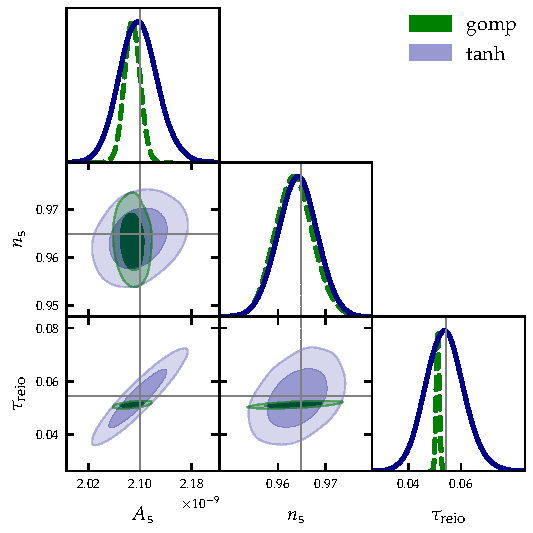
\includegraphics[width=0.6\linewidth]{figs/gomp_tanh_triangle_kill.pdf}
\caption{\textbf{Analysis of CMB data with reionization as a function of
cosmology.}
\YLtodo[inline]{contour and PDFs look quite big}
The green contours represent our results using the Gompertz reionization
model with \cref{eq:SR}, eliminating the need to sample over any
reionization parameter.
The blue contours correspond to the results obtained using the
conventional $\tanh$ model, while the relevant Planck constraints
\cite{Planck2020a} are depicted with gray lines for reference.}
\label{fig:kill}
\end{figure}

\Cref{fig:kill} underscores the impact of our universally-shaped
Gompertz reionization model.
The Gompertz model does not sample over reionization parameters but
maps cosmology parameters to $x_\HI$ profiles.\YL{too many repetitions?}
This approach tightens the constraint on the optical depth to $\approx
1\%$, a remarkable improvement compared to $> 10\%$ with the $\tanh$
prescription.
Furthermore, the constraint on $\As$ improves dramatically since the TT
data is no longer significantly hampered by the degeneracy between $\As$
and $\tau_\reio$.
The error on $\As$ decreases by an impressive factor of 2.5 compared to
Planck's results \cite{Planck2020a}.
Overall, we recover tighter constraints across the board compared to
Planck.
See \Cref{fig:unleashed_gomp} and \Cref{tab:para} in the Extended Data for details.


\section*{Outro}

\begin{figure}
\centering
\includegraphics[width=\linewidth]{figs/history.pdf}
\caption{\textbf{Reionization history $x_\HI$.}
Our best-fit Gompertz model (green dashed line) of Planck data is
asymmetric and differs significantly from that of the symmetric $\tanh$
model (blue lines, with dotted region representing the 1$\sigma$
errors).
Note $z$ is shown in logarithmic scale of $a^{-1}$.
We also include an alternative mapping from cosmology to Gompertz
timeline in the pink dotted line (see \nameref{ssec:0226}).
Additionally, we include observational constraints from high-redshift
quasars \cite{Greig2017, Banados2018, Davies2018, Greig2019, Wang2020,
Yang2020, Greig2022, Jin2023} and galaxies \cite{Ouchi2010,
Sobacchi2015, Mason2018, Mason2019, Hoag2019, Mesinger2015}.}
\YLtodo[inline]{Unify Gomp legend: gomp or Gomp or Gompertz}
\label{fig:history}
\end{figure}

Our results suggest that Planck data favors a delayed reionization
compared to other CMB-based constraints.
Our best-fit cosmological parameters indicate a midpoint of $z_\re =
7.40$ and a duration of $\Delta z \equiv z(x_\HI = 0.05) - z(x_\HI =
0.95) \sim 500 $ Myr.
While our results align with late reionization observations, the
difference from the $\tanh$ model is within 1$\sigma$.
The duration of reionization, though better suited to observational
constraints compared to the $\tanh$ model, might still be considered
somewhat rapid in the context of late reionization scenarios
\cite{Cain2021}.
\Cref{fig:history} illustrates the reionization timeline derived
from our best-fit values.

Our findings for the timeline of reionization align with late
reionization scenarios, which are supported by high-$z$ Lyman-$\alpha$
observations \cite{Keating2020, Cain2021}.
However, recent discoveries by JWST indicate the presence of massive,
bright galaxies at early redshifts $z \sim 10$
\cite{Adams2023, Bradley2023, Donnan2023}.
The presence of these early galaxies suggests a potential preference for
brighter galaxies to drive reionization, a role that in our
\texttt{21cmFAST} simulations was attributed to a population of faint
galaxies.

Furthermore, our results are influenced by the semi-numerical
prescription employed by \texttt{21cmFAST} to ionize the IGM, which,
while efficient and swift, could bias our findings.
Moreover, our exploration within the astrophysical framework of
\texttt{21cmFAST} has been limited to varying the ionization efficiency
(see \nameref{ssec:sims} in the Extended Data).
Therefore, a more comprehensive exploration is warranted to ensure, for
instance, that the rescaling tilt $\tilt$ remains a constant.
Additionally, a valuable exercise to refine the inherent relationship
between cosmological parameters and reionization history would involve
using more realistic, albeit slower, reionization models.
One such option is to use the THESAN simulations \cite{Kannan2022},
which are hydrodynamical simulations incorporating radiative transfer.


\paulo{Around 2000 words.}

\paulo{Body can only have 50 citations.}
